
\documentclass[
   12pt,                      % Schriftgroesse 12pt
   a4paper,                   % Layout fuer Din A4
   ngerman,                   % neue deutsche Rechtschreibung nach der Reform
   oneside,                   % Layout fuer einseitigen Druck
   headinclude,               % Kopfzeile wird Seiten-Layouts mit beruecksichtigt
   headsepline,               % horizontale Linie unter Kolumnentitel
   plainheadsepline,          % horizontale Linie auch beim plain-Style
   BCOR12mm,                  % Korrektur fuer die Bindung
   DIV18,                     % DIV-Wert fuer die Erstellung des Satzspiegels, siehe scrguide
   parskip=half,              % Absatzabstand statt Absatzeinzug
   openany,                   % Kapitel k�nnen auf geraden und ungeraden Seiten beginnen
   bibliography=totoc,        % Literaturverz. wird ins Inhaltsverzeichnis eingetragen
   toc=listof,                % Abbildungs- Tabellen- und sonstige verzeichnisse mit ins Inhaltsverzeichnis
   numbers=noenddot,          % Kapitelnummern immer ohne Punkt
   captions=tableheading,     % korrekte Abstaende bei TabellenUEBERschriften
     ]{scrbook}[2001/07/30]   % scrbook-Version mind. 2.8j von 2001/07/30

%##########################################################################################################
%
% Packete laden
%
%##########################################################################################################

\usepackage{ngerman}                           % neue Rechtschreibung
\usepackage[ansinew]{inputenc}                 % Input-Encodung: ansinew fuer Windows
\usepackage[T1]{fontenc}                       % T1-kodierte Schriften, korrekte Trennmuster fuer Worte mit Umlauten
\usepackage{ae}                                % F�r PDF-Erstellung
\usepackage[
	format=hang,
	font={footnotesize, sf},
	labelfont={bf},
	margin=1cm,
	aboveskip=5pt,
	belowskip=5pt
	]{caption,subfig}                            % mehrzeilige Captions ausrichten; subfig: Untergrafiken 

\usepackage[centertags]{amsmath}               % AMS-Mathematik, centertags zentriert Nummer bei split
\usepackage{amssymb}                           % zus�tzliche Symbole
\usepackage{trfsigns} 					               % f�r bestimmte Symbole
\usepackage{graphicx}                          % zum Einbinden von Grafiken
\usepackage[svgnames,table,hyperref]{xcolor}
\usepackage{float}                             % u.a. genaue Plazierung von Gleitobjekten mit H
\usepackage{epsfig}                            % eps Format f�r Grafiken
\usepackage[pdftex,pstarrows]{pict2e}
\usepackage{array}
\usepackage{listings}						               % Code-Einbindungsumgebung
\usepackage{courier}                           % verwende Courier statt cmtt als monospace-schrift
\usepackage{setspace}                          % Zeilenabstand einstellbar
\usepackage{rotating}
\onehalfspacing                                % eineinhalbzeilig einstellen
\usepackage{longtable}					               % Erm�glicht Tabellen die �ber den Seitenumbruch gehen (s. Symbolverzeichnis)
\usepackage{scrpage2}                          % Kopf und Fusszeilen-Layout passt besser zur Dokumentklasse KOMA-Skript (scrbook) als das Pake fancyhdr, sonst ziemlich gleichwertig
\usepackage{natbib}							               % Literaturzitate 
\typearea[current]{current}                    % Neuberechnung des Satzspiegels mit alten Werten nach �nderung von Zeilenabstand,etc
\usepackage{xcolor,colortbl}                   % Packet um Tabellen bunt auszuf�llen
\usepackage{wasysym}                           % Promillezeichen und co.
\usepackage{scrpage2}


%##########################################################################################################
%
% PDF-Erzeugung: pdflatex statt latex aufrufen! 
%
%##########################################################################################################

\pdfoutput=1              
\usepackage[pdftex,  % muss letztes Package sein!
     pdftitle={Titel der Arbeit},%
     pdfauthor={Vorname Nachname},%
     pdfsubject={Themen},%
     pdfkeywords={ ... },%
     pdfstartview={FitH},%
     pdfstartpage={5},%
     bookmarks,%
     raiselinks,%
     pageanchor,%
     hyperindex,%
     colorlinks,%
     citecolor=black!60!black,%
     linkcolor=black!70!black,%
     urlcolor=magenta!70!black,%
     filecolor=magenta!70!black,%
     menucolor=orange!70!black,%
    ]{hyperref}  

%##########################################################################################################
%
% New- and Renew-Commands
%
%##########################################################################################################


\renewcommand{\headfont}{\normalfont\sffamily}             % Kolumnentitel serifenlos
\renewcommand{\pnumfont}{\normalfont\ttfamily\bfseries}    % Seitennummern typewriter und fett 
\pagestyle{scrheadings}

% Einkommentieren falls beidseitige Darstellung erw�nscht!!! aktuell definiert: oneside -> Layout fuer einseitigen Druck

%\ihead[]{\headmark}              % Kolumnentitel immer oben innen   
%\ohead[\pagemark]{\pagemark}     % Seitennummern immer oben aussen
%\lefoot[]{} 
%\rofoot[]{}                      % Seitennummern in der Fusszeile loeschen

\newcommand {\jkarray}[1]{\ensuremath{\underline{#1}}} 
\newcommand {\jkmatrix}[1]{\ensuremath{\underline{\underline{#1}}}}
\newcommand {\einheit}[1]{\ensuremath{\mathrm{\left[#1\right]}}} 
\newcommand {\lived}[2]{($\ast$#1, $\dagger$#2)}  %


%###########################################################################################################
%
% Parameter f�r die jeweiligen Packete definieren
%
%###########################################################################################################

\lstdefinestyle{cppcode}{language={[Visual]C++},%
  basicstyle=\ttfamily\footnotesize,%
  keywordstyle={\color{Navy} \bfseries},%
  identifierstyle={\color{DarkRed}},%
  commentstyle={\color{DarkOrange!50!black}\slshape},%
  stringstyle={\color{DarkGreen}},%
  showstringspaces=false,%
  backgroundcolor={\color{LightSkyBlue!40}},%
  columns=fixed,%
  keepspaces=true,%
  basewidth={0.55em},%
  frame=shadowbox,%
  rulesepcolor=\color{Gray},%
  breaklines=true,%
  numbers=left,%
  numberstyle=\tiny,%
  escapeinside={�(}{)�},%
  moredelim={[is][\bfseries]{�^}{^�}},%
  belowcaptionskip=0.5cm%
  }%

\lstdefinestyle{fort}{language={[95]Fortran},%
  basicstyle=\ttfamily\small,%
  keywordstyle={\color{Navy} \bfseries},%
  identifierstyle={\color{DarkRed}},%
  commentstyle={\color{DarkOrange!50!black}\slshape},%
  stringstyle={\color{DarkGreen}},%
  showstringspaces=false,%
  backgroundcolor={\color{LightSkyBlue!40}},%
  columns=fullflexible,%
  keepspaces=true,%
  basewidth={0.6em},%
  rulesepcolor=\color{Gray},%
  frame=shadowbox,%
  escapeinside={�(}{)�},%
  moredelim={[is][\bfseries]{�^}{^�}},%
  belowcaptionskip=0.5cm%
  }%


\lstdefinestyle{pseudocode}{basicstyle=\ttfamily\small,%
  columns=fixed,%
  keepspaces=true,%
  basewidth={0.55em},%
  frame=shadowbox,%
  backgroundcolor={\color{LightSkyBlue!40}},%
  rulesepcolor=\color{Gray},%
  escapeinside={�(}{)�},%
  moredelim={[is][\bfseries]{�^}{^�}},%
  belowcaptionskip=0.5cm%
  }%

\lstdefinestyle{maple}{%
  basicstyle=\sffamily\small\color{Red}\bfseries,%
  rulecolor=\color{Black},%
  columns=fixed,%
  keepspaces=true,%
  basewidth={0.55em},%
  frame=shadowbox,%
  numbers=left,%
  numberstyle=\tiny\color{Black},%
  numberblanklines=false,%
  rulesepcolor=\color{Gray},%
  breaklines=true,%
  breakautoindent=true,%
  backgroundcolor={\color{LightBlue!60}},%
  rulesepcolor=\color{Gray},%
  escapeinside={�(}{)�},%
  moredelim={[is][\bfseries]{�^}{^�}},%
  belowcaptionskip=0.5cm%
  }%
  
\lstdefinestyle{matlab}{language={Matlab},%
  basicstyle=\ttfamily\small,%
  keywordstyle={\color{Navy} \bfseries},%
  identifierstyle={\color{DarkRed}},%
  commentstyle={\color{DarkOrange!50!black}\slshape},%
  stringstyle={\color{DarkGreen}},%
  showstringspaces=false,%
  backgroundcolor={\color{LightSkyBlue!30}},%
  breaklines=true,%
  breakautoindent=true,%
  columns=fullflexible,%
  keepspaces=true,%
  basewidth={0.6em},%
  rulesepcolor=\color{Gray},%
  frame=shadowbox,%
  numbers=left,%
  numberstyle=\tiny\color{Black},%
  escapeinside={�(}{)�},%
  moredelim={[is][\bfseries]{�^}{^�}},%
  belowcaptionskip=0.5cm%
  }%


\graphicspath{{figs/}{bilder/}{plots/}}    % Falls texinput nicht gesetzt -> Bildverzeichnisse
\setcitestyle{square,aysep={}}             % Eckige Klammern um Zitat

% hier sind Worte zu definieren die in der Worttrennung falsch oder nicht erkannt werden!

\hyphenation{Post-pro-cess-ing--In-te-gral}



%###########################################################################################################
%
% Aufbau des Dokuments -> Einf�gen der einzelnen Teile
%
%###########################################################################################################

% '''''''''''''''''''''''''''''''''''''''''''''''''''''''''''''''''''''
\newcommand{\sectionnumbering}[1]{%
  \setcounter{section}{0}%
   \renewcommand{\thesection}{\csname #1\endcsname{section}}}
% '''''''''''''''''''''''''''''''''''''''''''''''''''''''''''''''''''''

\newcounter{romanPagenumber} % neuen Seitenz�hler als Variable definieren
\begin{document}

\frontmatter

\setheadsepline{0.0pt} %Dicke der Trennlinie Kopfzeile - Text -> f�r Erkl�rungen ausschalten und erst ab Kurzzusammenfassung beginnen!

\pagenumbering{Roman}         % romanische Nummerierung f�r die Deckbl�tter, Inhaltsverzeichnis und co.

\begin{titlepage}

\begin{center}
{
%\fontsize{18}{18}\selectfont   % font Gr��e undefiniert-> es wird nur mit \text gearbeitet

\vspace*{-1.5cm}
\hfill \includegraphics*[width=3cm, keepaspectratio=true]{tumlogo}  
                       
\hrule                                 % horizontale Linie ein

\vspace{0.5cm} 

\textsc{\LARGE TECHNISCHE UNIVERSIT�T M�NCHEN}\\[2cm]

\textsc{\Large Lehrstuhl f�r Massivbau}\\[0.5cm]

\textsc{\Large Institut f�r Baustoffe und Konstruktion}\\[3.5cm]             

\textbf{\LARGE Vorlage und Guideline zur Erstellung einer Abschlussarbeit am Lehrstuhl f�r Massivbau - mit dem Programm LaTeX }\\[3.5cm]

\textsc{\Large Master�s Thesis im Studiengang Bauingenieurwesen}\\[3.5cm]


\textsc{Max Mustermann, B.Sc.} \\[2.5cm]
\textsc{M�nchen 2015} \\[0.5cm]


\vspace{3.5cm}
             

}
\end{center}

\end{titlepage}


\thispagestyle{empty}     % 2. Seite leer!
\section*{}

     % Deckblatt Titel

\begin{titlepage}

\begin{center}

{\fontsize{14pt}{14} 

\textsc{Master�s Thesis im Fach Massivbau} \\
\vspace{0.5cm}
\textsc{eingereicht an der Technischen Universit�t M�nchen}\\
\vspace{0.5cm}
\textsc{am Lehrstuhl f�r Massivbau}\\
\vspace{0.5cm}
\textsc{Institut f�r Baustoffe und Konstruktion}\\[3cm]

\textsc{\Large  \underline{Thema:}}\\[3.0cm]    
       
\textbf{\Large Vorlage und Guideline zur Erstellung einer Abschlussarbeit am Lehrstuhl f�r Massivbau - mit dem Programm LaTeX }\\[6cm]
}
{\fontsize{12pt}{12} \selectfont%
\begin{tabular}{ll}
Verfasser:& Nicholas Schramm, M.Sc.\\
Matrikelnummer:& 0815\\
Referent:& Univ.-Prof. Dr.-Ing. Dipl.-Wirt. Ing. Oliver Fischer\\
Betreuer:& Anna Musterfrau, M.Sc.\\[1cm]
Begonnen am:& 01.10.2015\\
Eingereicht:& \today\\
Abschlie�end beurteilt am:& 01.01.2016  \hspace{4cm} Note: \\
\end{tabular}                 
}
\end{center}

\end{titlepage}




     % Deckblatt detailiertere Bezeichnungen
\begin{titlepage}


\addchap{Erkl�rung}
\markboth{Erkl�rung}{Erkl�rung}
\label{cha:erkl}

Hiermit erkl�re ich, dass die vorliegende Master`s Thesis von mir selbst angefertigt wurde, und nur die aufgef�hrten Quellen und Hilfsmittel Verwendung fanden.
Ich erkl�re mich damit einverstanden, dass meine Master`s Thesis auf unbefristete Zeit zu Hochschulzwecken aufbewahrt werden darf.


\vfill
\vspace{2.5cm} 
M�nchen, \today \\
\vspace{2.0cm} \\
$\overline{\text{Max Mustermann, B.Sc.}}$
\vfill

\addchap{}
\label{cha:vakantseite}

\thispagestyle{empty}     % 2. Seite leer!
\section*{}

\end{titlepage}
        % Erkl�rung zur selbstst�ndigen Bearbeitung

\setheadsepline{0.5pt}        % Dicke der Trennlinie Kopfzeile - Text

\addchap{Kurzzusammenfassung}
\label{cha:Kurzzusammenfassung}

Die Kurzzusammenfassung dient der schnellen Information eines Lesers, der herausfinden m�chte, ob die
Inhalte der Arbeit f�r ihn von Interesse sind. Sie sollte in wenigen Zeilen einen m�glichst pr�zisen �berblick �ber die Arbeit
geben und in deutscher Sprache verfasst werden. % Kurzusammenfassung der Arbeit
\chapter{Abstract}
\label{cha:abtract} 

An abstract should be written in English language and be a greatly condensed version of your thesis that highlights the major points covered. It describes the content and scope of the writing. \\
Abstracts give readers a chance to quickly see what the main contents of your thesis are. They enable readers to decide whether the work is of interest for them.             % Abstract der Arbeit
\tableofcontents              % Inhaltsverzeichnis
\clearpage
\setcounter{romanPagenumber}{\value{page}} % eigener Seitenz�hler erh�lt aktuelle r�mische Seitenzahl

\mainmatter                   % den Hauptteil beginnen
\pagenumbering{arabic}        % ab hier wieder arabische Nummerierung
\chapter{Einleitung}
\label{kap:einleitung}

Die Einleitung ist ein sehr wichtiger Teil einer wissenschaftlichen Arbeit. Deshalb ist es wichtig, die Einleitung genau auf den Inhalt der Arbeit und ebenso auch auf das Fazit am Ende der Masterarbeit abzustimmen...          % Einleitung
\chapter{Kapitel, Unterkapitel und die Definitionen von Abschnitten}
\label{sec:Kapitel1}    % das Label ist nur wichtig f�r den Bezug auf das jeweilige Kapitel -> der Bezug wird mit \ref{sec:Kapitel1} aufgerufen (siehe Kapitel Beispiele)

\section{Abschnitt 1 meines ersten Kapitels}
\label{sec:Abschnitt1MeinesErstenKapitels}

\section{Abschnitt 2 meines ersten Kapitels}
\label{sec:Abschnitt2MeinesErstenKapitels}

\subsection{Unterabschnitt 1}
\label{sec:Unterabschnitt1}

\subsubsection{Unter-Unterabschnitt meines Unterabschnitts 1}
\label{sec:UnterUnterabschnittMeinesUnterabschnitts1}

Abschnitte, Unterabschnitte usw. lassen sich mit dem TeXnicCenter sehr einfach �ber Einf�gen $\rightarrow$ �berschrift oder durch die Tastenkombination Strg+Alt+S einf�gen. \\




            % Kapitel 1    
\section{Beispiele}
\label{sec:Beispiele}


\subsection{Beispiel f�r die Erstellung von Formeln}
\label{sec:Beispielf�rdieErstellungvonFormeln}

Formeln werden eingef�gt unter: Einf�gen $\rightarrow$ Formeln  \\
Die jeweiligen Unterschiede bei den m�glichen Typen lassen sich durch "`ausprobieren"' erlernen! \\

BEISPIEL:

..... Dabei kommt es durch die reduzierten Widerstandsmomente zu einer Erh�hung und durch die Minderung der elastischen L�nge zu einer Reduktion der L�ngsspannungen in der Schiene. Dies wird aus der in Kapitel \ref{sec:Kapitel1} hergeleiteten Gleichung f�r die maximale Schienenl�ngsspannung infolge einer vertikalen Einzellast ersichtlich:  

	\begin{equation}
		\sigma_{xx}=\frac{Q(\xi)\cdot \sqrt[4]{\frac{4\cdot E_{E} \cdot I_{E}}{b_{E}\cdot k}} \cdot 0,25}{W_{y_{unten}}} = \frac{Q(\xi)\cdot \sqrt[4]{\frac{4\cdot E_{E}}{b_{E}\cdot k}}\cdot z_{u}}{4 \cdot I_{E}^{0,75}}
		\label{eq:spannung_elast}
	\end{equation} 
	
Auf �hnliche Weise l�sst sich auch eine Matrix darstellen:

BEISPIEL:
	
...F�r ein Scheibenelement ergibt sich beispielsweise folgender Ansatz f�r die Diskretisierung des Verschiebungsfeldes:

\begin{equation}
\begin{bmatrix} u \\ v	\end{bmatrix}_{(e)} = \begin{bmatrix} \phi^{T}_{u}(x,y) & 0 \\ 0 & \phi^{T}_{v}(x,y)	\end{bmatrix}_{(e)} \begin{bmatrix} U_u \\ U_v	\end{bmatrix}_{(e)}	
\end{equation}
	
	
	
\subsection{Zitate einf�gen}
\label{sec:ZitateEinf�gen}

Als erstes ist es erforderlich die vorhandene Literatur in dem Programm "`Jabref"' einzutragen! Dies ist auf einfache Weise m�glich.Das Benutzerhandbuch findet sich unter 
\href{http://jabref.sourceforge.net/manuals/JabRef-UserManual_de.pdf} {Benutzerhandbuch - Jabref}

Zitate werden folgenderma�en eingef�gt: \citep{Bathe2002} \\
Es ist i.d.R. erforderlich hierf�r 3 mal nacheinander zu kompilieren bzw. das Dokument zu erstellen!\\
(Das Erstellen l�sst sich �brigens auch mit der Tastenkombination "`Strg+F5"' durchf�hren)\\
Nachdem die Quelle aufgerufen wurde, wird der entsprechende Eintrag im Literaturverzeichnis automatisch erstellt!

\subsection{Bilder einf�gen}
\label{sec:BilderEinf�gen}

Um Bilder einzuf�gen einfach das entsprechende Bild in dem Ordner "`bilder"' ablegen und wie folgt beschrieben einf�gen. Um den wunderbaren Vorteil von LaTeX zu nutzen, dass Vektorgrafiken eingebunden werden k�nnen, bitte das Bild in dem Format "`pdf"' abspeichern und eingescannte Bilder entsprechend mit hoher Qualit�t erstellen!

Bilder lassen sich einf�gen unter: Einf�gen $\rightarrow$ Grafik

Beispiel:

\begin{figure}[H]
	\centering
		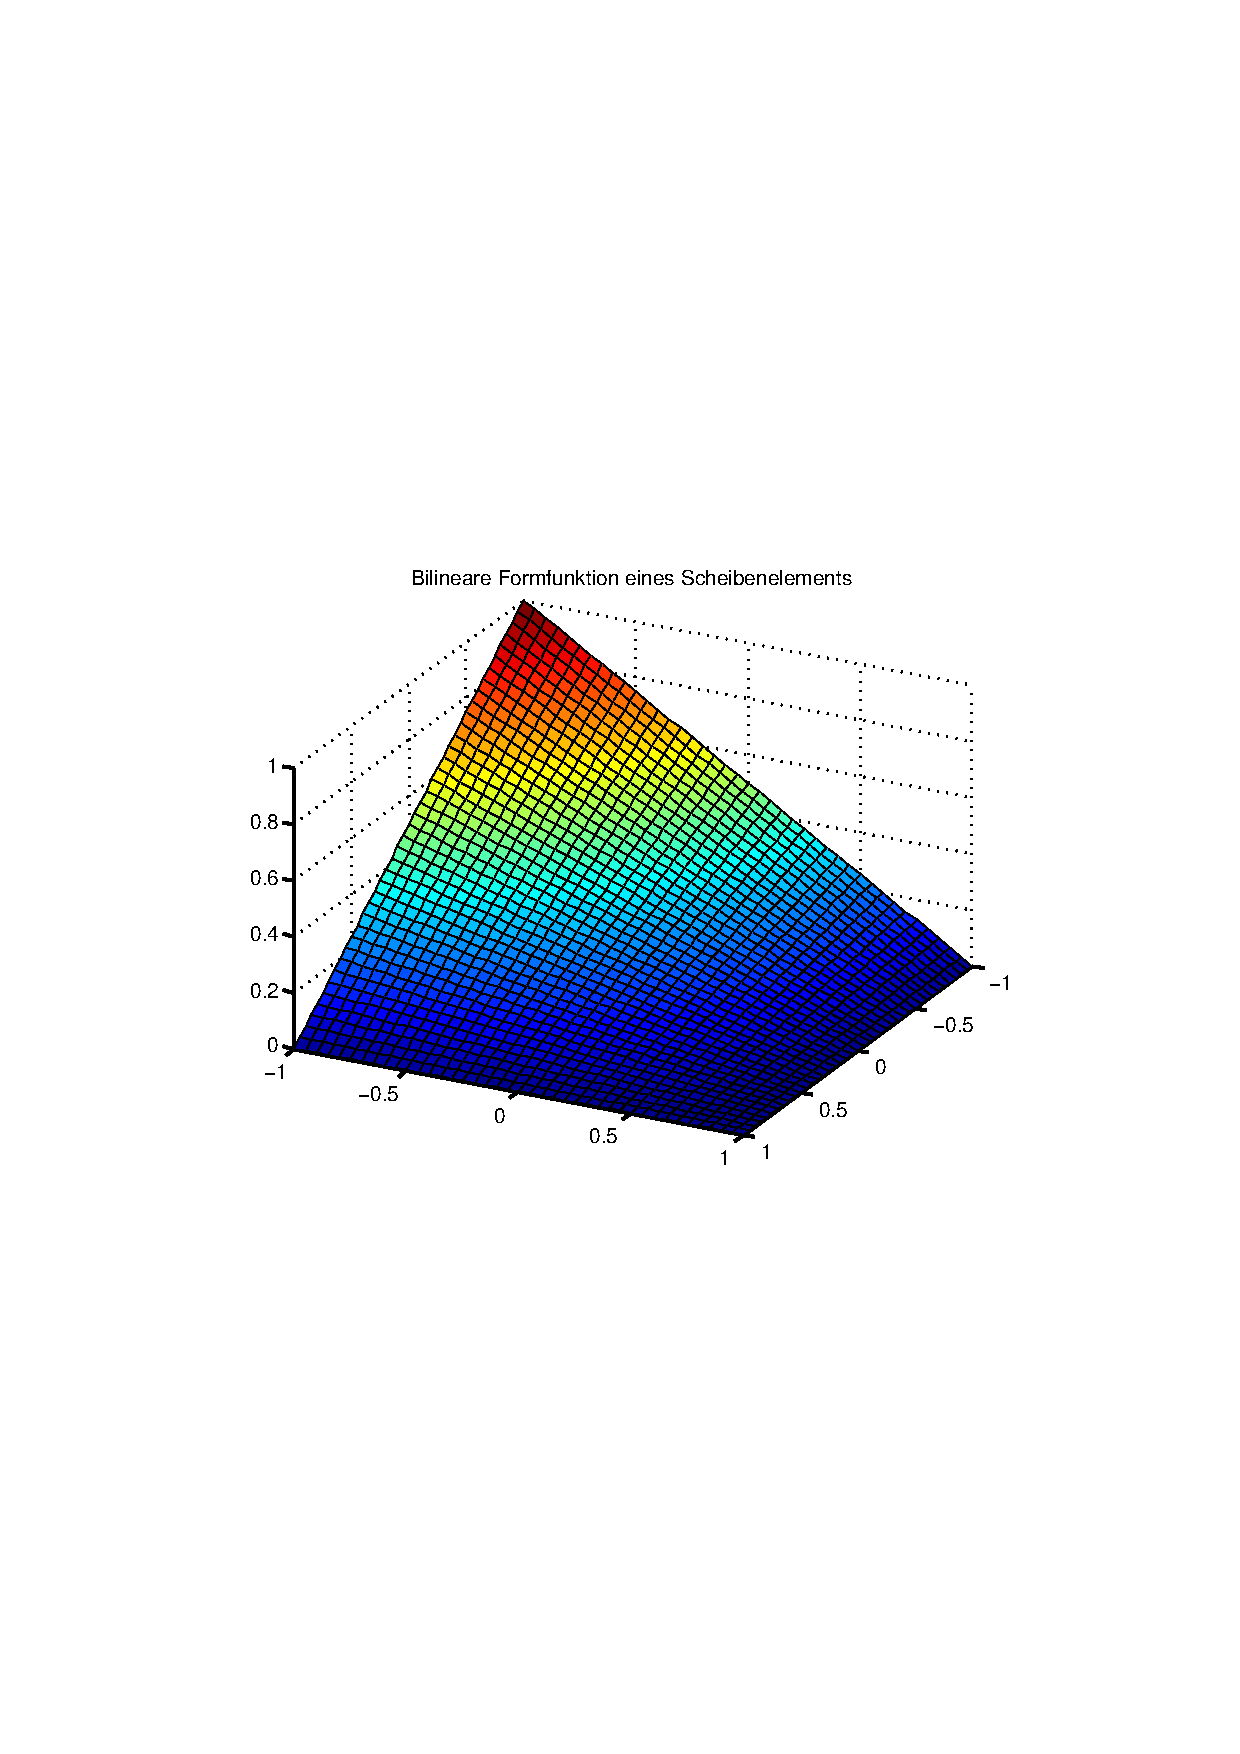
\includegraphics[width=0.4\textwidth]{bilder/140710_bilineare_Formfunktion.pdf}
	\caption{Beispielhafte Darstellung einer bilinearen Formfunktion f�r ein Scheibenelement}
	\label{fig:140710_bilineare_Formfunktion}
\end{figure}
Um den Unterschied zu einer "`Pixelgrafik"' zu sehen, einfach mal ganz weit in die Abbildung zoomen. Das Bild bleibt immer scharf!

\subsection{Tabellen einf�gen}
\label{sec:TabellenEinf�gen}

Tabellen werden unter Tabelle $\rightarrow$ einf�gen erstellt!

Beispiel:

\begin{table} [H]
\centering
\caption{Versuchsergebnisse zur Ermittlung der Federsteifigkeiten der elastischen Zwischenplatte Zwp BSP FF-B-1; Zulassungspr�fungen an der TU M�nchen}
\begin{tabular}{|c|c|c|c|} \hline  
\rowcolor[gray]{.9} 
 Pr�ftemperatur & stat. Steifigkeit $c_{stat}$ & dyn. Steifigkeit $c_{dyn}$ & Pr�ffrequenz \\\hline 
\rowcolor[gray]{.9} 
 $[�C]$                & $[kN/mm]$ & $[kN/mm]$ & $[Hz]$ \\\hline 
 50  & 33,6 & -    & -           \\\hline 
 50  & -    & 42,1 & 10        \\\hline
 23  & 33,0 & -    & -           \\\hline 
\end{tabular} 
\label{tab:Steifigkeiten_Zwp_TUM}
\end{table}


Beispiel "`Farbig"':

Nachfolgend ein Beispiel zum Erstellen von farbigen Tabellen:

\definecolor{LightCyan}{rgb}{0.88,1,1}           % Definieren der gew�nschten Farben
\definecolor{leichtesGelb}{rgb}{0.9,0.9,0}
\definecolor{maroon}{cmyk}{0,0.87,0.68,0.32}

\begin{table} [H]
\centering
\caption{Beispiel farbige Tabelle}
\begin{tabular}{|c|c|c|c|} \hline  
\rowcolor[gray]{.9} 
 Lastfallnr. & Bezeichnung des Modells & max. $w_{zz}$ (vertikal) & max. $v_{yy}$ (horizontal) \\\hline 
\rowcolor[gray]{.9} 
 $[-]$ & $[-]$ & $[mm]$ & $[mm]$ \\\hline 

\rowcolor{LightCyan}
\textcolor{red} 1 & {Stabwerk mit 5 Stp.}  & \textcolor{red} {1,86} & \textcolor{red} {0,00}    \\\hline 
\rowcolor{LightCyan}
1 & Volumen mit 5 Stp.  & 1,85 & 0,00     \\\hline 
\rowcolor{LightCyan}
\textcolor{red} 1 & {Stabwerk mit 6 Stp.}  & \textcolor{red} {1,87} & \textcolor{red} {0,00}   \\\hline 
\rowcolor{LightCyan}
1 & Volumen mit 6 Stp.  & 1,89 & 0,00   \\\hline 

\rowcolor{leichtesGelb!20}
\textcolor{red} 2 & {Stabwerk mit 5 Stp.}  & \textcolor{red} {1,86} & \textcolor{red} {0,34}    \\\hline 
\rowcolor{leichtesGelb!20}
2 & Volumen mit 5 Stp.  & 1,90 & 0,41     \\\hline
\rowcolor{leichtesGelb!20}
\textcolor{red} 2 & {Stabwerk mit 6 Stp.}  & \textcolor{red} {1,87} & \textcolor{red} {0,32}   \\\hline 
\rowcolor{leichtesGelb!20}
2 & Volumen mit 6 Stp.  & 1,91 & 0,36   \\\hline 

\textcolor{red} 3 & {Stabwerk mit 5 Stp.}  & \textcolor{red} {1,61} & \textcolor{red} {3,56}    \\\hline 
3 & Volumen mit 5 Stp.  & 1,64 & 3,25    \\\hline 
\textcolor{red} 3 & {Stabwerk mit 6 Stp.}  & \textcolor{red} {1,62} & \textcolor{red} {3,57}   \\\hline 
3 & Volumen mit 6 Stp.  & 1,65 & 3,31  \\\hline 
\end{tabular}

\label{tab:farbigeTabelle} 
\vspace{0.0cm}
\end{table} 



Die Tabellen werden automatisch in das Tabellenverzeichnis eingetragen!

\section{Sonstiges}
\label{sec:Sonstiges}

F�r weitere Informationen ist die "`LaTeX Kurzbeschreibung"' vom Leibniz Rechenzentrum sehr hilfreich: \href{https://www.lrz.de/services/software/textverarbeitung/tex/l2kurz.pdf} {Benutzerhandbuch - LaTeX} \\
Um Schnell etwas zu suchen, ist es zumeist am einfachsten das Zeichen oder das Problem zu "`googlen"'. Zur Erstellung von Arbeiten mit LaTeX gibt es unz�hlige Foren usw.

Viel Erfolg und Spa� beim Erstellen der Arbeit!














 
	            % Kapitel 1  
\chapter{Zusammenfassung}
\label{sec:zusammenfassung}

Ziel dieser Arbeit war es, ...     % Zusammenfassung
\appendix                     % Anhang

\chapter{Anhang}
\label{cha:anhang}


\clearpage

 
\backmatter

\pagenumbering{Roman}                    % f�r letzte Verzeichnisse wieder romanische Nummerierung
\sectionnumbering{Roman}
\setcounter{page}{\theromanPagenumber}   % setzt die aktuelle Seitenzahl von vorne f�r die romanische Nummerierung fest 
\listoffigures                           % Abbildungsverzeichnis
\listoftables


\newpage
\addchap{Symbolverzeichnis}
\markboth{Symbolverzeichnis}{Symbolverzeichnis}
\label{cha:symbolverzeichnis}


\begin{longtable}[l]{lcp{8cm}l}
$E$ & \einheit{\frac{N}{mm^{2}}} & Elastizit�tsmodul\\
\end{longtable}                        % Symbolverzeichnis    

 \bibliographystyle{natdin}
 \bibliography{bibliothek}

\end{document}


